\subsection{Fernsteuerung}
\label{subsec:fernsteuerung}

Der letzte Schritt zur vollständigen Steuerung des \gls{go1} aus der Ferne ist die Fernsteuerung der Bewegungen des
Roboters.
Hierfür muss geprüft werden, inwiefern sich die Befehle der Fernbedienung aus Kapitel \ref{subsec:fernsteuerung}
über ein Netzwerk replizieren lassen.
Die Ergebnisse aus den Kapiteln \ref{subsubsec:led} und \ref{subsubsec:batterie-management} lassen vermuten, dass sich
die Bewegung über MQTT steuern lässt.

\myparagraph{Analyse der Webseite}

Eine Inspektion des Quellcodes der Webseite zeigt folgenden Ausschnitt der Datei \texttt{webpack\allowbreak :///\allowbreak src/\allowbreak views/\allowbreak Vision.vue}.

\begin{lstlisting}[
    numbers=left,xleftmargin=\dimexpr3em-1pt,framexleftmargin=2.5em,
    firstnumber=172,
    label={lst:vision-vue},caption=Ausschnitt der Datei \texttt{Vision.vue}
]
const handleStickData = (evt: {
    lx: number;
    ly: number;
    rx: number;
    ry: number;
}) => {
    const floats = new Float32Array(4);
    floats[0] = evt.lx;
    floats[1] = evt.rx;
    floats[2] = evt.ry;
    floats[3] = evt.ly;
    mqtt.publish("controller/stick", floats.buffer, { qos: 0 });
};
\end{lstlisting}

Die Ausgabe der Zeilen \num{173} bis \num{176} lässt vermuten, dass die beiden Joysticks der Fernbedienung emuliert werden,
in dem $x$ und $y$ Werte angegeben werden, um die Position des Sticks relativ zum Nullpunkt - der Mitte - zu errechnen.
Über das Bewegen des linken Sticks der auf der Webseite angezeigten Steuerungen auf ein oberes Maximum lässt sich über
das Einhängen eines Debuggers folgender Wert der vier Koordinaten ausgeben.

\begin{lstlisting}
evt = {lx: 0,ly: 1,rx: 0,ry: 0}
\end{lstlisting}

\noindent Die möglichen Float-Werte der Koordinaten können also zwischen \num{-1} und \num{1} liegen.
Die Dokumentation der Implementierung der JavaScript-Klasse \texttt{Float32Array} zeigt, dass das Array \texttt{floats}
in Zeile \num{178} vier Floats mit der Länge \num{32} bit speichert.
Die Funktion \texttt{floats.buffer} in Zeile \num{183} schreibt die vier Werte in binärer Representation in den Message
Payload des MQTT Topics \texttt{controller/stick}.
Um nun die Werte \texttt{lx=0}, \texttt{ly=1}, \texttt{rx=0} und \texttt{ry=0} manuell an den MQTT Broker des \gls{go1} zu
senden, müssen die Werte in ihre binäre Form und die richtige Reihenfolge gebracht werden.
Die Zeilen \num{179} bis \num{182} zeigen, dass die korrekte Reihenfolge der binären Koordinaten der Steuerung
\texttt{lx \textrightarrow rx \textrightarrow ry \textrightarrow ly} ist.

Zum Test der Ergebnisse kann ein Befehl mit dem Paket \texttt{mosquitto\_pub} an den Broker gesendet werden.
Hierfür ist die hexadezimale Darstellung der Werte hilfreich.
Die hexadezimale Representation des binären Wertes eines \texttt{float32} mit dem Wert \num{1} ist Folgende.

\begin{lstlisting}
Binaer  = 00111111100000000000000000000000
Hex     = 3F800000
\end{lstlisting}

\noindent Der Befehl lautet wie folgt.

\begin{lstlisting}
echo -ne "\x00\x00\x00\x00\x00\x00\x00\x00\x00\x00\x00\x00\x3f\x80\x00\x00" | mosquitto_pub -h 192.168.123.161 -t controller/stick -s
\end{lstlisting}

\noindent Da man die Stellung der zwei Sticks dauerhaft konfiguriert, sollte man die Werte zum Test schnellstmöglich
wieder auf null zurücksetzen, da der Roboter im Beispiel oben sonst dauerhaft vorwärtsläuft.

\myparagraph{Aufbau der Fernsteuerung}

Da die Komplexität einer gesamten Anwendung für dieses Beispiel über den Rahmen der Arbeit hinaus geht, soll hier nur kurz
ein Diagramm der nötigen Komponenten für eine minimale Anwendung zur Fernsteuerung des Roboters dargestellt werden.

\begin{figure}[h]
    \frame{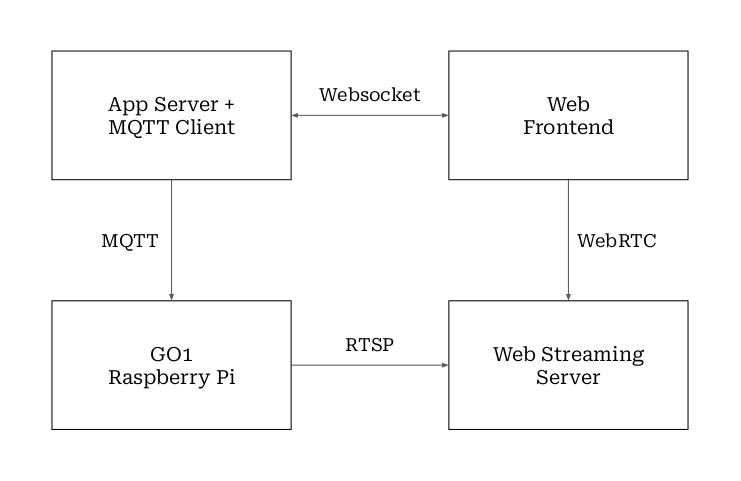
\includegraphics[width=\linewidth]{img/erweiterung/remote}}
    \caption{Diagramm der Komponenten einer beispielhaften Fernsteuerungssoftware}\label{fig:remote}
\end{figure}

\noindent Als Grundlage für die Anwendung dient ein Appserver, welcher sowohl eine Websocket mit MQTT-Anbindung bereitstellt,
als auch die Webseite hostet, welche die Steuerung und einen optionalen Videostream der Kamerabilder des Roboters enthält.
Die Webseite sendet per Websocket die Nutzereingaben an den Server, wobei dieser die Eingaben in MQTT-Messages umwandelt
und diese an den Broker im Raspberry Pi des \gls{go1} sendet.

\myparagraph{Integration des Videostreams}

\gls{html} unterstützt in den meisten modernen Browsern nativ die Übertragung von \gls{webrtc} Streams.
Dies wurde bereits in Kapitel \ref{subsec:remote-video-streaming} gezeigt.
Auch das native \gls{html} Tag \texttt{<video/>} kann diese Streams einbetten.
Hierfür muss lediglich das Attribut \texttt{src} mit der \gls{url} des Streams auf dem Streaming-Server gesetzt werden.

Wie in Abbildung \ref{fig:remote} gezeigt, kann nun die Webseite mit dem eingebetteten Stream über die Verwendung des
nativen \gls{html} Tags \texttt{<video/>} direkt auf den Streaming-Server zugreifen und somit nicht nur die Steuerung,
sondern auch die Kamerabilder anzeigen.
Für die Funktion der Fernsteuerung und der integrierten Videoübertragung müssen alle in Abbildung \ref{fig:remote} gezeigten
Komponenten im selben Netzwerk sein oder über mehrere Netzwerke hinweg miteinander kommunizieren können.
Die Vorbereitungen aus den Kapiteln \nameref{subsubsec:wifi} und \nameref{subsubsec:gsm} können hierfür hilfreich sein.